\documentclass[11pt,a4paper]{article}
\usepackage[utf8]{inputenc}
\usepackage[T1]{fontenc}
\usepackage[english]{babel}
\usepackage[margin=2.1cm]{geometry}
\usepackage{booktabs,array,tabularx}
\usepackage{xcolor}
\usepackage{graphicx}
\usepackage{pgfplots}
\pgfplotsset{compat=1.17}
\PassOptionsToPackage{hyphens}{url}
\usepackage[hidelinks]{hyperref}
\usepackage{enumitem}
\setlist{nosep,leftmargin=1.4em}
\emergencystretch=3em

\definecolor{impl}{HTML}{3B6EA8}
\definecolor{rev}{HTML}{8FB3DA}

\title{Sweatshop on P-Chess: the v0.1.0 review, history and home screens\\\large Review screen (REV-005), summary and graph (REV-006), history (HIST-004), delete (HIST-005), analysis queue (HIST-006), home (UI-016), searching (UI-017), your name (UI-018) and profile (UI-019); GPT-6.1 Terra lineup with a Sol fallback, lane \texttt{v010}, run 3}
\author{Foreman, session \texttt{sweatshop/v010/2026-10-30-2302}}
\date{31 October 2026}

\begin{document}
\maketitle

\section*{Summary}

Run 3 of the \texttt{v010} lane in its clone at \path{.artifacts-build/lanes/v010}, resuming the
session of run 2 (PR \href{https://github.com/Laginho/P-Chess/pull/28}{\#28}). Bruno was asleep
and had given the parent session every call for the night; the parent set the starting decisions
(below), the foreman took the routine ones and the proxy the contract one. Launch at 23:29, last
merge at 03:15.

\begin{itemize}
  \item \textbf{Produced:} all nine remaining \texttt{v010} tickets merged on the session with
        \texttt{Verdict: Approve}: REV-005 (\texttt{Review: human}, reviewed tonight by the agent
        in Bruno's place, as he allowed), REV-006, HIST-004, HIST-005, HIST-006, UI-016, UI-017,
        UI-018, UI-019. The lane has nothing left. Gate 400 passed, 0 failed (337 before the run).
  \item \textbf{Cost:} \textbf{\$20.66} at API list price over 34 stages, all priced: review
        \texttt{gpt-6.1-sol xhigh} \$11.49 (15), \texttt{gpt-6.1-terra high} \$2.70 (9),
        \texttt{gpt-6.1-terra xhigh} \$2.70 (5), \texttt{gpt-6.1-sol high} \$3.09 (4),
        \texttt{gpt-6.1-sol xhigh} implementing \$0.68 (1). Codex quota: 6 points of the weekly
        window (Sol xhigh 4, Terra xhigh 1, Sol high 1, Terra high 0; $\pm$1 each), no reset;
        4 Codex rollouts ran outside the stages (the desktop app), 0 points.
  \item \textbf{What went wrong:} Terra high stopped early three times (HIST-004 twice, UI-017
        once): one red/green pair, then a progress report instead of a handoff. The foreman's one
        restart moved HIST-004 to Terra xhigh, which finished it; at UI-017's stop the run
        switched to the Sol lineup, as authorized. A driver parse defect parked HIST-005's valid
        handoff once. Six reviews reopened, all real findings.
  \item \textbf{Provisional verdict:} Terra xhigh finishes big tickets (4 of 4 first stage-2 runs
        to review, 11--12~min); Terra high does not reliably (3 early stops in 7 first attempts).
        Sol high finished the last three tickets on its first attempt each.
\end{itemize}

Parent decisions applied before launch: merge \texttt{main} (the Godot binding,
\texttt{1427740}) into the session; REV-005 to \texttt{Difficulty: hard} with a comment to resume
from run 2's \texttt{f5e9337} and finish every criterion; default lineup with an authorized Sol
fallback after one diagnosis and restart.

\section*{What was done}

\textbf{REV-005}: the new review screen. The board, a vertical eval bar, the move list beside it
with a class icon on each move once its class is settled, and the engine's best-move arrow.
Opening a review runs the Max analysis and fills icons as positions land, reusing a saved
analysis when there is one. Partial analysis comes from a new mode in
\path{core/classification.gd} (proxy decision of run 2). Main files \path{ui/review.gd},
\path{ui/eval_bar.gd}, \path{ui/board_view.gd}. Reopened once: with the review open, \texttt{F}
flipped the hidden game board instead of the review board, and the eval bar did not follow
(\path{ui/review.gd}).

\textbf{REV-006}: the review's summary: accuracy per side, class counts, an interactive eval
graph that jumps to a move when clicked, and help tooltips. Main file \path{ui/review.gd}.
Reopened once: the tooltips opened 1241 and 3517~px wide at 800$\times$600, off the window.

\textbf{HIST-004}: the history screen. Tabs (All, wins, losses, draws), game cards with a
thumbnail, colours, result and cached accuracy; a card opens its game in the review; the default
tab is a setting. Main files \path{ui/history_screen.gd}, \path{core/history.gd}. Merged at the
first review, which fixed one crash itself: opening History before the first saved game failed
on the missing folder.

\textbf{HIST-005}: delete a game, after a confirmation: the PGN and its analysis and snapshot
files go, and the result, flag and practice counters are reversed; a failed removal restores
files and counts. PGNs gain \texttt{PracticeTarget}. Main files \path{core/history.gd},
\path{ui/history_screen.gd}. Reopened twice: the rollback repairs had no red/green test (proxy:
provoke the failures through the filesystem, no new seam); then, after HIST-006 merged, deleting
a game the queue was analysing let the analyser write its JSON back
(\path{ui/history_screen.gd} now cancels the queued analysis).

\textbf{HIST-006}: a background analysis queue, saved across restarts, one game at a time, with
priority for the game being reviewed and pause during play; History shows the batch progress.
Main files \path{core/analysis_queue.gd}, \path{ui/history_screen.gd}. Reopened once: the
post-game review ignored a valid saved analysis and started over, and the status lacked
``2 of 7''.

\textbf{UI-016}: the app opens on a home screen: quick play with the saved choices, Custom game
(the old setup screen), History and Settings. Main file \path{ui/main.gd}. Merged at the first
review.

\textbf{UI-017}: a searching screen covers the wait for Maia (at least 0.5~s, until
\texttt{readyok}) before the game starts; engine failures report there. Main file
\path{ui/main.gd}. Terra high stopped early on it; Sol high implemented it from scratch and it
merged at the first review.

\textbf{UI-018}: the app asks your name once and writes it, with \texttt{HumanColor}, to every
PGN; history and deletion identify you by that colour, and old PGNs fall back as before. Main
files \path{ui/name_dialog.tscn}, \path{core/pgn.gd}. Reopened once: the name field overlapped
the question in the dialog.

\textbf{UI-019}: a profile screen: rename yourself, your results table from the history
counters, and a chart of your dated accuracy. Merged at the first review.

\section*{Timeline}

{\small
\begin{tabularx}{\linewidth}{@{}lX@{}}
\toprule
23:2x & Parent decisions applied: \texttt{main} merged into the session (\texttt{0a7aa75}); REV-005 hard, resume comment (\texttt{d5d14eb}). \\
23:29 & Launch, default lineup (Terra), pid 29940. \\
23:42 & REV-005 to review (Terra xhigh, 12~min, resumed from \texttt{f5e9337}). \\
23:47--23:55 & REV-005 reopened (F flips the hidden board), fixed in 4~min, merged. \\
00:05--00:16 & REV-006 to review, reopened (tooltip width), fixed, merged. \\
00:20--00:21 & HIST-004: Terra high stops early, then stops on the recovered commits: blocked. \\
00:22 & Foreman diagnosis, the run's one restart: HIST-004 hard, resume from \texttt{2c6272b} (\texttt{8ce8bdd}); pid 2204. \\
00:34--00:40 & HIST-004 to review (Terra xhigh, 11~min), merged; the review fixed one crash itself. \\
00:49--00:57 & HIST-005 to review, reopened (no red/green for the rollbacks); the fix asks the proxy (00:54), the proxy decides (00:57). \\
01:02 & HIST-005's fix reaches \texttt{to-review}, but the driver parks it (parse defect). \\
01:13--01:27 & HIST-006 to review (Terra xhigh), reopened (cache, batch status), fixed, merged. \\
01:45--01:52 & UI-016 to review (Terra high, 18~min), merged at the first review. \\
01:54 & UI-017: Terra high stops early after 2~min; nothing runnable. \\
01:55 & Foreman: HIST-005's review note reworded (\texttt{cc3ee76}), \texttt{to-review} restored; UI-017 diagnosis (\texttt{8780914}); relaunch on \texttt{-Lineup sol}, pid 4876. \\
02:03 & HIST-005 reopened a second time (integration with HIST-006); the driver parks it for diagnosis. \\
02:18--02:22 & UI-017 to review (Sol high, 15~min), merged; nothing runnable. \\
02:22 & Foreman diagnosis of HIST-005 (\texttt{476aee7}); relaunch on Sol, pid 29148. \\
02:32--02:35 & HIST-005 to review (Sol xhigh, 9~min), merged. \\
02:49--03:02 & UI-018 to review (Sol high), reopened (dialog overlap), fixed, merged. \\
03:12--03:15 & UI-019 to review (Sol high, 10~min), merged. Nothing left; PR \#28 (9 tickets). \\
\bottomrule
\end{tabularx}
}

\section*{Per stage}

{\small
\begin{tabularx}{\linewidth}{@{}llllrrrrrX@{}}
\toprule
When & Ticket & Stage & Model & Min & In & Cache & Out & Cost & Outcome \\
\midrule
23:42 & REV-005 & impl & terra xhigh & 12 & 10.4M & 99\% & 24k & 0.78 & to-review \\
23:47 & REV-005 & review & sol xhigh & 5 & 3.8M & 94\% & 18k & 0.99 & reopened \\
23:51 & REV-005 & impl & terra xhigh & 4 & 2.4M & 97\% & 5k & 0.21 & to-review \\
23:55 & REV-005 & review & sol xhigh & 4 & 2.5M & 95\% & 12k & 0.62 & merged \\
00:05 & REV-006 & impl & terra high & 10 & 5.2M & 97\% & 16k & 0.50 & to-review \\
00:09 & REV-006 & review & sol xhigh & 4 & 2.4M & 94\% & 15k & 0.67 & reopened \\
00:13 & REV-006 & impl & terra high & 4 & 1.9M & 97\% & 5k & 0.17 & to-review \\
00:16 & REV-006 & review & sol xhigh & 3 & 1.9M & 93\% & 11k & 0.57 & merged \\
00:20 & HIST-004 & impl & terra high & 3 & 2.1M & 95\% & 4k & 0.24 & failed \\
00:21 & HIST-004 & impl & terra high & 1 & 0.2M & 81\% & 1k & 0.05 & failed, blocked \\
00:34 & HIST-004 & impl & terra xhigh & 11 & 11.0M & 99\% & 26k & 0.78 & to-review \\
00:40 & HIST-004 & review & sol xhigh & 7 & 4.9M & 96\% & 19k & 1.03 & merged \\
00:49 & HIST-005 & impl & terra high & 9 & 5.2M & 99\% & 15k & 0.38 & to-review \\
00:53 & HIST-005 & review & sol xhigh & 3 & 2.2M & 92\% & 11k & 0.65 & reopened \\
00:54 & HIST-005 & impl & terra high & 1 & 0.4M & 89\% & 2k & 0.08 & asked \\
01:02 & HIST-005 & impl & terra high & 5 & 3.3M & 98\% & 8k & 0.28 & parked$^{*}$ \\
01:13 & HIST-006 & impl & terra xhigh & 11 & 9.2M & 99\% & 26k & 0.69 & to-review \\
01:19 & HIST-006 & review & sol xhigh & 6 & 4.2M & 95\% & 22k & 1.01 & reopened \\
01:24 & HIST-006 & impl & terra xhigh & 5 & 2.4M & 97\% & 8k & 0.23 & to-review \\
01:27 & HIST-006 & review & sol xhigh & 3 & 2.0M & 93\% & 10k & 0.55 & merged \\
01:45 & UI-016 & impl & terra high & 18 & 13.1M & 99\% & 26k & 0.89 & to-review \\
01:52 & UI-016 & review & sol xhigh & 7 & 4.4M & 96\% & 17k & 0.96 & merged \\
01:54 & UI-017 & impl & terra high & 2 & 1.1M & 96\% & 7k & 0.13 & failed, blocked \\
02:03 & HIST-005 & review & sol xhigh & 6 & 4.9M & 96\% & 20k & 1.05 & reopened \\
02:18 & UI-017 & impl & sol high & 15 & 5.7M & 98\% & 30k & 1.13 & to-review \\
02:21 & UI-017 & review & sol xhigh & 3 & 3.1M & 93\% & 12k & 0.82 & merged \\
02:32 & HIST-005 & impl & sol xhigh & 9 & 3.5M & 97\% & 15k & 0.68 & to-review \\
02:35 & HIST-005 & review & sol xhigh & 4 & 2.4M & 93\% & 12k & 0.66 & merged \\
02:49 & UI-018 & impl & sol high & 14 & 4.1M & 98\% & 25k & 0.84 & to-review \\
02:53 & UI-018 & review & sol xhigh & 4 & 3.3M & 95\% & 13k & 0.77 & reopened \\
02:59 & UI-018 & impl & sol high & 6 & 2.1M & 97\% & 7k & 0.41 & to-review \\
03:02 & UI-018 & review & sol xhigh & 3 & 1.4M & 92\% & 10k & 0.46 & merged \\
03:12 & UI-019 & impl & sol high & 10 & 3.1M & 96\% & 19k & 0.72 & to-review \\
03:15 & UI-019 & review & sol xhigh & 4 & 2.5M & 93\% & 11k & 0.68 & merged \\
\midrule
 & & & & 216 & 132.3M & & 482k & 20.66 & \\
\bottomrule
\end{tabularx}
}

\noindent$^{*}$ The run log says \texttt{failed (incomplete handoff), blocked}; the stage in fact
reached \texttt{to-review} with a valid gate receipt (366/0). The driver misread the receipt
field (see Driver and runtime issues).

\begin{center}
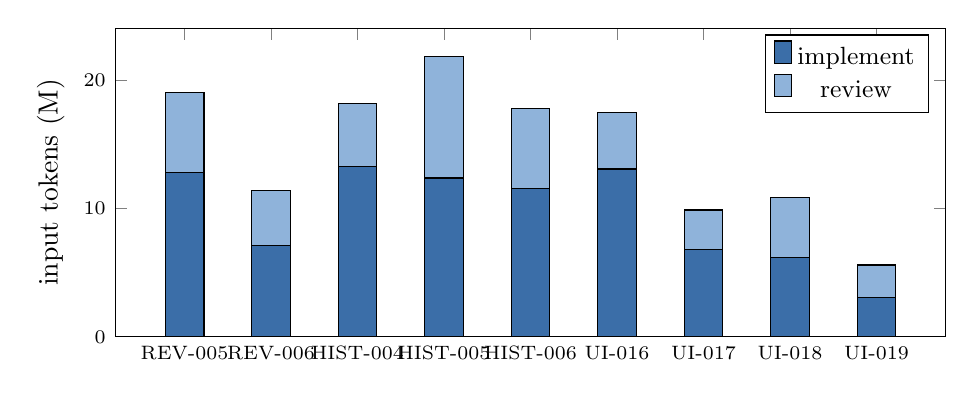
\begin{tikzpicture}
\begin{axis}[ybar stacked, bar width=14pt, width=\linewidth, height=5.5cm,
  symbolic x coords={REV-005,REV-006,HIST-004,HIST-005,HIST-006,UI-016,UI-017,UI-018,UI-019},
  xtick=data, ylabel={input tokens (M)}, ymin=0, legend style={at={(0.98,0.98)},anchor=north east,font=\small},
  tick label style={font=\scriptsize}]
\addplot[fill=impl] coordinates {(REV-005,12.8) (REV-006,7.1) (HIST-004,13.3) (HIST-005,12.4) (HIST-006,11.6) (UI-016,13.1) (UI-017,6.8) (UI-018,6.2) (UI-019,3.1)};
\addplot[fill=rev] coordinates {(REV-005,6.3) (REV-006,4.3) (HIST-004,4.9) (HIST-005,9.5) (HIST-006,6.2) (UI-016,4.4) (UI-017,3.1) (UI-018,4.7) (UI-019,2.5)};
\legend{implement, review}
\end{axis}
\end{tikzpicture}
\end{center}

Wasted: the three early stops (HIST-004 2.3M in, \$0.28; UI-017 1.1M, \$0.13), HIST-005's proxy
ask (0.4M, \$0.08), and the six rejected first attempts with their reviews. HIST-005's parked
fix was not wasted: its work was kept and reviewed. Dollars go mostly to review: \$11.49 of
\$20.66.

\section*{Comparison with previous runs}

From \texttt{run-log.md}. Run~1 of this lane (5 tickets, Terra unpriced) and run~2 (REV-005 only,
4 failed or parked stage 2s, \$0.63) set the baseline. Tonight the first stage 2 took 10--18~min
on Terra high when it finished (REV-006, HIST-005, UI-016), 11--12~min on Terra xhigh (REV-005,
HIST-004, HIST-006), and 10--15~min on Sol high (UI-017, UI-018, UI-019), against Sol high's
scoreboard median of 9~min to review. Fixes after a reopen took 4--9~min on every model. Reviews
cost \$0.46--1.05 (\$0.66--1.21 in run~1). Per merged ticket the run cost \$2.30.

\section*{Observations per model}

\begin{itemize}
  \item \textbf{gpt-6.1-terra high, stage 2} (9 stages, 4 tickets): when it finished, it finished
        well: REV-006, HIST-005 and UI-016 opened with red tests, green gates, honest handoffs.
        But 3 of its 7 first attempts across runs 2--3 were early stops (HIST-004 after one pair;
        UI-017 after one test, with uncommitted work), the same failure as REV-005 in run~2. Its
        second HIST-004 attempt read the recovered commits as work it must not continue and
        stopped without changes. HIST-005's first handoff carried two rollback fixes without
        tests. UI-016's quick-play tests wrote eight fake games into the real \path{user://}
        history; it noticed, backed them up, removed exactly those eight games and their stats
        entry, and isolated the test (foreman checked: the 28 real games are intact).
  \item \textbf{gpt-6.1-terra xhigh, stage 2} (5 stages, 3 tickets): every first attempt reached
        review, on the three largest tickets of the run (REV-005 +533 lines, HIST-004 +560,
        HIST-006 +471), resuming saved work when told to. Two of three were reopened, each for
        a regression next to its own change (F flip, cache reuse) plus a stated criterion.
  \item \textbf{gpt-6.1-sol high, stage 2} (4 stages, 3 tickets): three first attempts to review,
        one reopen (UI-018 layout). On UI-017 it adapted the 14 old tests that the delayed start
        broke, where Terra had stopped. Slower and dearer per stage than Terra high
        (\$0.72--1.13).
  \item \textbf{gpt-6.1-sol xhigh, review} (15 stages, 3--7~min): every reopen was probed and
        real; no noise, no drip-feed (HIST-005's second finding came from HIST-006's new code, and
        the review said so). It fixed one crash itself in HIST-004 with a red/green pair and an
        independent review. It ran the gate after rebases and reused receipts otherwise.
\end{itemize}

\section*{Driver and runtime issues}

\begin{enumerate}
  \item \texttt{GateEvidenceField} (\path{driver.ps1:214}) takes the first line that matches
        \texttt{Gate evidence:}. HIST-005's round-1 review wrote a bullet ``- Gate evidence:
        reused the supplied receipt\dots'' above stage 2's field, so the driver passed that prose
        to \texttt{Get-Content -LiteralPath \dots{} -Raw}, which failed (``A parameter cannot be
        found that matches parameter name Raw''), and parked a valid \texttt{to-review} as
        \texttt{incomplete handoff}. Once this run; it can recur on any reopen whose review uses
        that wording.
  \item Terra high ends its turn with a progress report on big tickets. The driver counts it as
        a failed attempt (exit 0, Stage not \texttt{to-review}); the second attempt then sees the
        recovery commits and may stop on them.
  \item The Stockfish binary is not in the lane clone, so REV-005, HIST-006 and UI-017 could not
        exercise the real engine; their handoffs say so.
  \item Tests write into the real \path{user://} folder: \texttt{test\_*} folders, an analysis JSON
        from HIST-005's tests and an empty \texttt{analysis\_queue.cfg} from HIST-006's remain there.
  \item Shutdown 0.8--1.8~s per stage; no crash, no timeout, no API error.
\end{enumerate}

\section*{Recommendations}

\begin{enumerate}
  \item Fix \texttt{GateEvidenceField} to take the last match, or the first whose value is a
        path that exists; keep the self-check cases at \path{driver.ps1:822--825}.
  \item Do not run Terra high on tickets that span several files and screens: give them
        \texttt{Difficulty: hard} (Terra xhigh) or run Sol high. Implementer rows:
        \texttt{gpt-6.1-terra high} 28 stage runs, 10 failed, 2 asked; \texttt{gpt-6.1-terra
        xhigh} 11 runs, 0 failed; \texttt{gpt-6.1-sol high} 68 runs, 0 failed.
  \item Make the tests use an isolated user folder throughout (UI-016 did it for its own test),
        and clean the leftovers in \path{AppData/Roaming/Godot/app_userdata/[P] Chess}.
  \item Put interacting tickets in each other's \texttt{Blocked by} (HIST-005 and HIST-006 touch
        the same analysis files), so the later one is written against the earlier one's code.
  \item Before tagging, play the manual checks below with real Stockfish.
\end{enumerate}

\section*{Human debt and proxy decisions}

No \texttt{Débito humano:} lines in this run's tickets. One proxy decision, on HIST-005, asked by
the driver after stage 2 stopped on the question:

\begin{itemize}
  \item \texttt{Proxy decided (opus-5.5 xhigh)}: ``No new production seam. Stage 2 provokes the
        failures from the filesystem, the way \path{tests/test_history.gd:411} already does. The
        reason: no contract change, it follows the repo's existing pattern, and only
        \path{tests/test_history.gd} (a Primary file) changes.''
\end{itemize}

Decisions taken for Bruno without the proxy, by the parent session and the foreman: REV-005 to
\texttt{hard} with a resume comment; HIST-004 to \texttt{hard} with a resume comment; the switch
to the Sol lineup at UI-017; REV-005's \texttt{Review: human} covered by the agent review tonight.

\section*{Reopen attribution}

Labelled by the foreman (opus-5.5); the reviewer was \texttt{gpt-6.1-sol xhigh}, so no
self-judging. Rows appended to \path{.scratch/reopen-attribution.md}.

{\small\noindent
\begin{tabularx}{\linewidth}{@{}>{\raggedright\arraybackslash}p{1.7cm}X>{\raggedright\arraybackslash}p{2.7cm}X@{}}
\toprule
Ticket (round) & Finding & Label & Why \\
\midrule
REV-005 (1) & \texttt{F} flips the hidden game board; the eval bar does not follow & S2-implícito & regression of its own change; the repo already flips with F \\
REV-006 (1) & Tooltips 1241 and 3517~px wide at 800$\times$600 & S2-explícito/\allowbreak código & criterion 4 names the minimum window; left as manual \\
HIST-005 (1) & Rollback repairs without red/green proof & S2-explícito/\allowbreak teste & test-first; nothing failed with the repairs reverted \\
HIST-005 (2) & Deleting a game being analysed lets the analyser rewrite its JSON & S1 ? & the queue merged after HIST-005 was written and reviewed; planning gap, borderline S2 \\
HIST-006 (1) & Post-game review ignores a valid saved analysis & S2-implícito & regression against REV-005's cache reuse \\
HIST-006 (1) & Status lacks the batch position ``2 of 7'' & S2-explícito/\allowbreak código & criterion 3 \\
UI-018 (1) & Name field overlaps the question & S2-explícito/\allowbreak código & criterion 1; layout untested \\
HIST-004 (0) & History fails before the first saved game & S2-implícito & fixed in review; failure path of its own screen \\
\bottomrule
\end{tabularx}
}

Totals, reopens: S2-explícito/código 3, S2-explícito/teste 1, S2-implícito 2, S1 1 (borderline),
S3-ruído 0; fixed in review: 1 S2-implícito. No review miss, no review-induced churn, no
drip-feed. No session-review, release-audit or post-release finding recorded yet for PR \#28.

\section*{Scoreboard}

\texttt{scoreboard.ps1} over the ClassyCall, EasyMath, PhysiSyst, SIGAA-ME and SynchroNice main
checkouts plus this lane's clone in place of P-Chess's main checkout (same merged run log; it
holds this run's attribution rows before they reach \texttt{main}). Moved since run~1's report:
implementer \texttt{gpt-6.1-terra high} 10 $\to$ 28 stage runs, 1 $\to$ 10 failed, 0 $\to$ 2
asked; \texttt{gpt-6.1-terra xhigh} 1 $\to$ 11 runs, 0 failed; pair \texttt{gpt-6.1-terra high}
$\rightarrow$ \texttt{gpt-6.1-sol xhigh} 9 $\to$ 16 reviews, 33\% $\to$ 31\% (S2 rate 31\%);
\texttt{gpt-6.1-terra xhigh} $\rightarrow$ \texttt{gpt-6.1-sol xhigh} 1 $\to$ 10 reviews, 30\%;
\texttt{gpt-6.1-sol high} $\rightarrow$ \texttt{gpt-6.1-sol xhigh} 18 $\to$ 22 reviews, 22\%
$\to$ 23\%. Both Terra pairs now have 10 or more reviews; their reopen rates are about 8 points
above Sol high's under the same reviewer. Interventions: automatic-recovery 89 $\to$ 101,
proxy-decision (opus-5.5 xhigh) 1 $\to$ 6 (other lanes included).

{\tiny
\begin{verbatim}
| Implementer | Stage runs | To review | Failed | Asked | Median min to review | Cost |
|---|---|---|---|---|---|---|
| gpt-6.1-sol high | 68 | 63 | 0 | 5 | 9m | $52.36 (68/68 priced) |
| opus-5.5 medium | 3 | 2 | 1 | 0 | 6m | $4.79 (3/3 priced) |
| opus-5.5 | 7 | 4 | 0 | 3 | 14m | $15.12 (7/7 priced) |
| gpt-6-luna max | 89 | 61 | 10 | 18 | 17m | $4.91 (85/89 priced) |
| sonnet-5.5 high | 2 | 2 | 0 | 0 | 7m | $3.77 (2/2 priced) |
| gpt-6-astra high | 1 | 0 | 0 | 1 | - | $3.92 (1/1 priced) |
| opus-5.5 xhigh | 18 | 14 | 4 | 0 | 12m | $91.78 (18/18 priced) |
| gpt-6.1-sol max | 6 | 5 | 0 | 1 | 24m | $12.12 (6/6 priced) |
| gpt-6-sol xhigh | 1 | 1 | 0 | 0 | 9m | $0.40 (1/1 priced) |
| fable | 1 | 1 | 0 | 0 | 11m | ? |
| gpt-6-luna | 8 | 4 | 4 | 0 | 37m | ? |
| gpt-6-sol | 6 | 5 | 1 | 0 | 17m | ? |
| gpt-5.6-sol | 5 | 4 | 1 | 0 | 17m | ? |
| gpt-6-astra | 18 | 11 | 6 | 1 | 8m | ? |
| sonnet | 5 | 3 | 2 | 0 | 14m | $10.53 (4/5 priced) |
| sonnet-5 xhigh | 11 | 6 | 2 | 3 | 8m | $18.09 (11/11 priced) |
| haiku-5.5 high | 2 | 0 | 2 | 0 | - | $1.00 (2/2 priced) |
| opus-5.5 high | 20 | 13 | 6 | 1 | 6m | $37.46 (20/20 priced) |
| gpt-6.1-sol xhigh | 10 | 10 | 0 | 0 | 12m | $10.52 (10/10 priced) |
| gpt-6.1-terra high | 28 | 16 | 10 | 2 | 8m | $3.49 (14/28 priced) |
| gpt-6.1-terra xhigh | 11 | 10 | 0 | 1 | 9m | $2.70 (5/11 priced) |

| Implementer | Reviewer | Reviews | Reopened | Reopen rate | Reopened for S2 | S2 rate | Unclassified | Fixed in review for S2 |
|---|---|---|---|---|---|---|---|---|
| gpt-6.1-sol high | gpt-6.1-sol max | 38 | 12 | 32% | 9 | >=24% | 2 | 1 |
| opus-5.5 medium | gpt-6.1-sol max | 2 | 1 | 50% | 0 | >=0% | 1 | 0 |
| opus-5.5 | opus-5.5 | 4 | 0 | 0% | 0 | 0% | 0 | 0 |
| gpt-6-luna max | opus-5.5 high | 18 | 1 | 6% | 1 | 6% | 0 | 0 |
| gpt-6-luna max | gpt-6-sol max | 43 | 23 | 53% | 22 | 51% | 0 | 0 |
| ? | gpt-6-sol max | 1 | 0 | 0% | 0 | 0% | 0 | 0 |
| sonnet-5.5 high | gpt-6-sol max | 2 | 1 | 50% | 1 | 50% | 0 | 0 |
| opus-5.5 xhigh | gpt-6.1-sol max | 6 | 3 | 50% | 3 | 50% | 0 | 0 |
| ? | gpt-6.1-sol max | 1 | 0 | 0% | 0 | 0% | 0 | 0 |
| gpt-6.1-sol max | gpt-6.1-sol max | 4 | 1 | 25% | 1 | 25% | 0 | 0 |
| gpt-6-sol xhigh | gpt-6-astra high | 1 | 0 | 0% | 0 | 0% | 0 | 0 |
| fable | fable | 1 | 1 | 100% | 0 | >=0% | 1 | 0 |
| ? | opus | 1 | 0 | 0% | 0 | 0% | 0 | 0 |
| gpt-6-luna | gpt-6-sol | 4 | 4 | 100% | 0 | >=0% | 4 | 0 |
| gpt-6-sol | gpt-5.6-sol | 5 | 4 | 80% | 0 | >=0% | 4 | 0 |
| gpt-5.6-sol | gpt-6-astra | 4 | 3 | 75% | 0 | >=0% | 3 | 0 |
| gpt-6-astra | gpt-5.6-sol | 11 | 5 | 45% | 0 | >=0% | 5 | 0 |
| sonnet | opus | 3 | 1 | 33% | 1 | 33% | 0 | 0 |
| sonnet-5 xhigh | opus-5.5 xhigh | 5 | 0 | 0% | 0 | 0% | 0 | 0 |
| ? | opus-5.5 xhigh | 4 | 1 | 25% | 1 | 25% | 0 | 0 |
| opus-5.5 xhigh | opus-5.5 xhigh | 7 | 0 | 0% | 0 | 0% | 0 | 0 |
| opus-5.5 high | opus-5.5 xhigh | 10 | 2 | 20% | 2 | 20% | 0 | 3 |
| gpt-6.1-sol high | gpt-6.1-sol xhigh | 22 | 5 | 23% | 5 | 23% | 0 | 0 |
| gpt-6.1-sol xhigh | gpt-6.1-sol xhigh | 10 | 1 | 10% | 1 | 10% | 0 | 1 |
| gpt-6.1-terra high | gpt-6.1-sol xhigh | 16 | 5 | 31% | 5 | 31% | 0 | 0 |
| ? | gpt-6.1-sol xhigh | 2 | 1 | 50% | 0 | 0% | 0 | 0 |
| gpt-6.1-terra xhigh | gpt-6.1-sol xhigh | 10 | 3 | 30% | 3 | 30% | 0 | 1 |

| Implementer -> Reviewer | Rounds | S2 explicit code | S2 explicit test | S2 implicit | S1 | S3 noise |
|---|---|---|---|---|---|---|
| gpt-6-astra medium -> gpt-6.1-sol max | 8 | 11 | 1 | 4 | 1 | 0 |
| gpt-6.1-sol-fast high -> gpt-6.1-sol-fast max | 2 | 2 | 0 | 0 | 0 | 0 |
| gpt-6.1-sol-fast max -> gpt-6.1-sol-fast max | 6 | 2 | 0 | 3 | 1 | 0 |
| gpt-6.1-sol high -> gpt-6.1-sol max | 26 | 16 | 4 | 23 | 1 | 0 |
| gpt-6-luna max -> opus-5.5 high | 1 | 1 | 1 | 0 | 1 | 0 |
| gpt-6-luna max -> gpt-6-sol max | 23 | 31 | 3 | 23 | 12 | 15 |
| sonnet-5.5 high -> gpt-6-sol max | 1 | 3 | 0 | 2 | 0 | 0 |
| opus-5.5 xhigh -> gpt-6.1-sol max | 3 | 3 | 0 | 2 | 1 | 0 |
| gpt-6.1-sol max -> gpt-6.1-sol max | 5 | 7 | 0 | 5 | 0 | 0 |
| haiku-5.5 high -> gpt-6.1-sol max | 3 | 3 | 1 | 5 | 1 | 0 |
| gpt-6.1-sol high -> gpt-6.1-sol xhigh | 54 | 54 | 4 | 23 | 3 | 0 |
| gpt-6.1-sol max -> gpt-6.1-sol xhigh | 2 | 0 | 0 | 3 | 0 | 0 |
| opus-5.5 high -> opus-5.5 xhigh | 8 | 7 | 0 | 3 | 0 | 0 |
| gpt-6.1-sol xhigh -> gpt-6.1-sol xhigh | 3 | 4 | 0 | 1 | 0 | 0 |
| opus-5.5 high -> gpt-6.1-sol xhigh | 1 | 2 | 0 | 0 | 0 | 0 |
| sonnet-5.5 high -> gpt-6.1-sol max | 3 | 5 | 0 | 2 | 3 | 0 |
| sonnet-5.5 xhigh -> gpt-6.1-sol max | 3 | 7 | 0 | 3 | 2 | 0 |
| sonnet-5.5 high -> opus-5.5 xhigh | 3 | 1 | 2 | 0 | 0 | 0 |
| gpt-6-astra medium -> gpt-6-astra xhigh | 1 | 1 | 0 | 0 | 0 | 0 |
| fable -> ? | 4 | 5 | 1 | 3 | 1 | 0 |
| sonnet -> ? | 10 | 3 | 6 | 9 | 3 | 2 |
| opus -> ? | 1 | 3 | 0 | 0 | 0 | 0 |
| sonnet? -> ? | 11 | 3 | 4 | 12 | 3 | 5 |
| sonnet -> opus | 1 | 1 | 1 | 0 | 0 | 0 |
| gpt-6-astra low -> gpt-6.1-sol max | 1 | 2 | 0 | 1 | 0 | 0 |
| gpt-6.1-terra high -> gpt-6.1-sol xhigh | 6 | 6 | 1 | 3 | 1 | 0 |
| gpt-6.1-terra xhigh -> gpt-6.1-sol xhigh | 4 | 4 | 0 | 3 | 0 | 0 |

Evidence coverage: legacy flags and absent records are unknown, not zero defects or zero interventions.
| Discovery | Recorded findings | Earlier review miss (yes / known) | Review-induced churn (yes / known) |
|---|---|---|---|
| ticket-review | 383 | 5 / 188 | 1 / 190 |
| session-review | 30 | 23 / 25 | 0 / 29 |
| release-audit | 2 | 2 / 2 | 0 / 2 |
Runtime completion to process exit: 314.119s total over 250 measured stages; 334 unmeasured.
| Intervention | Recorded events |
|---|---|
| human-rescue | 30 |
| automatic-recovery | 101 |
| proxy-decision (unknown) | 37 |
| routine-approval | 18 |
| proxy-decision (gpt-6-astra high, fallback) | 58 |
| proxy-decision (opus) | 42 |
| proxy-decision (supervisor) | 12 |
| proxy-decision (opus-5.5 xhigh) | 6 |
\end{verbatim}
}

\section*{Pending for the human}

\begin{enumerate}
  \item Review and merge session PR \#28 (9 tickets). REV-005 was \texttt{Review: human}; the agent
        review stood in tonight, so read its diff first.
  \item Play the v0.0.2 checks with real Stockfish: open a review after a game (icons arrive,
        eval bar, arrow, \texttt{F} flips board and bar, 800$\times$600); the summary, graph clicks
        and tooltips; History tabs, a card into the review and \texttt{Esc} back; delete a game,
        including one the queue is analysing; queue pause during a game and resume after a
        restart; home quick play and Custom game; the searching screen; the name dialog on first
        start and the name in PGNs; the profile rename, table and chart.
  \item Fix the driver's \texttt{GateEvidenceField} (recommendation 1) and decide Terra high's
        place in the lineup (recommendation 2).
  \item Clean the test leftovers in the real \path{user://} folder; the eight test games are
        backed up in \path{%TEMP%/p-chess-ui016-history-backup} if anything looks missing.
\end{enumerate}

\end{document}
